\let\negmedspace\undefined
\let\negthickspace\undefined
\documentclass[journal,12pt,onecolumn]{IEEEtran}
\usepackage{cite}
\usepackage{amsmath,amssymb,amsfonts,amsthm}
\usepackage{algorithmic}
\usepackage{graphicx}
\graphicspath{{./figs/}}
\usepackage{textcomp}
\usepackage{xcolor}
\usepackage{txfonts}
\usepackage{listings}
\usepackage{enumitem}
\usepackage{mathtools}
\usepackage{gensymb}
\usepackage{comment}
\usepackage{caption}
\usepackage[breaklinks=true]{hyperref}
\usepackage{tkz-euclide} 
\usepackage{listings}
\usepackage{gvv}                                        
%\def\inputGnumericTable{}                                 
%\usepackage[latin1]{inputenc}     
\usepackage{xparse}
\usepackage{color}                                            
\usepackage{array}                                            
\usepackage{longtable}                                       
\usepackage{calc}                                             
\usepackage{multirow}
\usepackage{multicol}
\usepackage{hhline}                                           
\usepackage{ifthen}                                           
\usepackage{lscape}
\usepackage{tabularx}
\usepackage{array}
\usepackage{float}
\newtheorem{theorem}{Theorem}[section]
\newtheorem{problem}{Problem}
\newtheorem{proposition}{Proposition}[section]
\newtheorem{lemma}{Lemma}[section]
\newtheorem{corollary}[theorem]{Corollary}
\newtheorem{example}{Example}[section]
\newtheorem{definition}[problem]{Definition}
\newcommand{\BEQA}{\begin{eqnarray}}
\newcommand{\EEQA}{\end{eqnarray}}
\newcommand{\define}{\stackrel{\triangle}{=}}
\theoremstyle{remark}
\newtheorem{rem}{Remark}

\setlength{\tabcolsep}{15pt}
\renewcommand{\arraystretch}{1.75}

\begin{document}

\title{GATE 2019-CE}
\author{Pratyush Panda(AI25BTECH11024)}
\maketitle

\renewcommand{\thefigure}{\theenumi}
\renewcommand{\thetable}{\theenumi}

\section*{General Aptitude(GA)}
\section*{Q. 1-Q. 5 carry one mark each.}

\begin{enumerate}

\item The lecture was attended by quite \underline{\hspace{2cm}} students, so the hall was not very \underline{\hspace{2cm}}.

\hfill{\brak{\text{GATE CE 2019}}}
\begin{enumerate}
\item a few, quite
\item few, quiet
\item a few, quiet
\item few, quite
\end{enumerate}

\item They have come a long way in \underline{\hspace{2cm}} trust among the users.

\hfill{\brak{\text{GATE CE 2019}}}
\begin{enumerate}
\item creating
\item created
\item creation
\item create
\end{enumerate}

\item On a horizontal ground, the base of a straight ladder is $6m$ away from the base of the vertical pole. The ladder makes an angle of $45^\circ$ to the horizontal. If the ladder is resting at a point located at one-fifth of the height of the pole from the bottom, the height of the pole is \underline{\hspace{2cm}} meters.

\hfill{\brak{\text{GATE CE 2019}}}
\begin{enumerate}
\item 15
\item 25
\item 30
\item 35
\end{enumerate}

\item If $E=10$; $J=20$; $O=30$; and $T=40$, what will be $P+E+S+T$?

\hfill{\brak{\text{GATE CE 2019}}}
\begin{enumerate}
\item 51
\item 82
\item 120
\item 164
\end{enumerate}

\item The CEO's decision to quit was as shocking to the Board as it was to \underline{\hspace{1cm}}.

\hfill{\brak{\text{GATE CE 2019}}}
\begin{enumerate}
\item I
\item me
\item my
\item myself
\end{enumerate}

\section*{Q. 6-Q. 10 carry two marks each.}

\item The new cotton technology, Bollgard-II, with herbicide tolerant traits has developed into a thriving business in India. However, the commercial use of this technology is not legal in India. Notwithstanding that, report indicate that the herbicide tloerant Bt cotton had been purchased by farmers at an average of Rs 200 more than the control price of ordinary cotton, and planted in $15\%$ of the cotton growing area in the 2017 Kharif season.\\
Which one of the following statements can be inferred from the given paragraph?

\hfill{\brak{\text{GATE CE 2019}}}
\begin{enumerate}
\item Farmers want to access the new technology if India benefits from it
\item Farmers want to access the new technology even if its not legal
\item Farmers want to access the new technology for experimental purpose
\item Farmers want to access the new technology by paying high prices
\end{enumerate}

\item In a sports academy of 300 people, 105 play only cricket, 70 play only hockey, 50 play only football, 25 play both cricket and hockey, 15 play both hockey and football and 30 play both cricket and football. The rest of them play all three sports. What is the percentage of people who play at least two sports?

\hfill{\brak{\text{GATE CE 2019}}}
\begin{enumerate}
\item 23.30
\item 25.00
\item 28.00
\item 50.00
\end{enumerate}

\item The increasing interest in tribal characters might be a mere coincidence, but the timing is of interest. None of this, though, is to say that the tribal hero has arrived in Hindi cinema, or that the new crop of characters represents the acceptance of the tribal character in the industry. The films and characters are too few to be described as a pattern.\\
What does the word `arrived' mean in the paragraph above?

\hfill{\brak{\text{GATE CE 2019}}}
\begin{enumerate}
\item reached a terminus
\item came to a conclusion
\item attained a status
\item went to a place
\end{enumerate}

\item A square has sides $5cm$ smaller than the sides of a second square. The area of the larger square is four times the area of the smaller square. The side of the larger square is \underline{\hspace{2cm}} cm.

\hfill{\brak{\text{GATE CE 2019}}}
\begin{enumerate}
\item 18.50
\item 15.10
\item 10.00
\item 8.50
\end{enumerate}

\item P, Q, R, S and T are related and belong to the same family. P is the brother of S. Q is the wife of P. R and T are the children of the siblings P and S respectively. Which one of the following statements is necessarily FALSE?

\hfill{\brak{\text{GATE CE 2019}}}
\begin{enumerate}
\item S is the aunt of R
\item  S is the aunt of T
\item S is the sister-in-law of Q
\item  S is the brother of P
\end{enumerate}

\section*{END OF THE QUESTION PAPER}
\end{enumerate}

\section*{Q. 1-Q. 25 carry one mark each.}

\begin{enumerate}
\item Which one of the following is correct?

\hfill{\brak{\text{GATE CE 2019}}}
\begin{enumerate}
\item $\lim_{x \to 0} \left(\frac{\sin 4x}{\sin 2x}\right) = 2$ and $\lim_{x \to 0} \left(\frac{\tan x}{x}\right) = 1$
\item $\lim_{x \to 0} \left(\frac{\sin 4x}{\sin 4x}\right) = 1$ and $\lim_{x \to 0} \left(\frac{\tan x}{x}\right) = 1$
\item $\lim_{x \to 0} \left(\frac{\sin 4x}{\sin 2x}\right) = \infty$ and $\lim_{x \to 0} \left(\frac{\tan x}{x}\right) = 0$
\item $\lim_{x \to 0} \left(\frac{\sin 4x}{\sin 2x}\right) = 2$ and $\lim_{x \to 0} \left(\frac{\tan x}{x}\right) = \infty$
\end{enumerate}

\item Consider a two-dimensional flow through isotropic soil along $x$ direction and $z$ direction. If $h$ is the hydraulic head, the Laplace’s equation of continuity is expressed as

\hfill{\brak{\text{GATE CE 2019}}}
\begin{enumerate}
\item $\frac{\partial h}{\partial x} + \frac{\partial h}{\partial z} = 0$
\item $\frac{\partial h}{\partial x} + \frac{\partial h}{\partial z} + \frac{\partial h}{\partial z} = 0$
\item $\frac{\partial^2 h}{\partial x^2} + \frac{\partial^2 h}{\partial z^2} = 0$
\item $\frac{\partial^2 h}{\partial x^2} + \frac{\partial^2 h}{\partial z} + \frac{\partial^2 h}{\partial z^2} = 0$
\end{enumerate}

\item A simple mass-spring oscillatory system consists of a mass $m$, suspended from a spring of stiffness $k$. Considering $z$ as the displacement of the system at any time $t$, the equation of motion for the free vibration of the system is $m\ddot{z} + kz = 0$. The natural frequency of the system is

\hfill{\brak{\text{GATE CE 2019}}}
\begin{enumerate}
\item $\frac{k}{m}$
\item $\sqrt{\frac{k}{m}}$
\item $\frac{m}{k}$
\item $\sqrt{\frac{m}{k}}$
\end{enumerate}
\item For a small value of $h$, the Taylor series expansion for $f(x+h)$ is

\hfill{\brak{\text{GATE CE 2019}}}
\begin{enumerate}
\item[(A)] $f(x) + hf'(x) + \frac{h^2}{2!}f''(x) + \frac{h^3}{3!}f'''(x) + \ldots \infty$
\item[(B)] $f(x) - hf'(x) + \frac{h^2}{2!}f''(x) - \frac{h^3}{3!}f'''(x) + \ldots \infty$
\item[(C)] $f(x) + hf'(x) + \frac{h^2}{2}f''(x) + \frac{h^3}{3}f'''(x) + \ldots \infty$
\item[(D)] $f(x) - hf'(x) + \frac{h^2}{2}f''(x) - \frac{h^3}{3}f'''(x) + \ldots \infty$
\end{enumerate}

\item A plane truss is shown in the figure $\brak{\textit{not drawn to scale}}$

\begin{figure}[H]
\centering
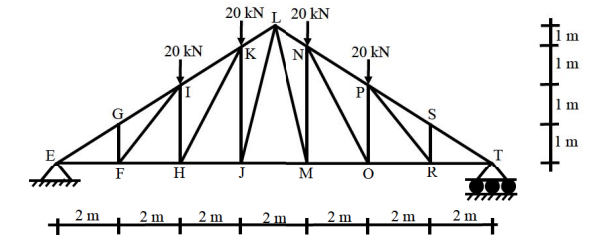
\includegraphics[width=0.5\columnwidth]{figs/q5.png}
\caption*{}
\label{fig:Q.5}
\end{figure}
Which one of the options contains ONLY zero force members in the truss?

\hfill{\brak{\text{GATE CE 2019}}}
\begin{enumerate}
\item FG, FI, HI, RS
\item FG, FH, HI, RS
\item FI, HI, PR, RS
\item FI, FG, RS, PR
\end{enumerate}

\item An element is subjected to biaxial normal tensile strains of $0.0030$ and $0.0020$. The normal strain in the plane of maximum shear strain is

\hfill{\brak{\text{GATE CE 2019}}}
\begin{enumerate}
\item Zero
\item $0.0010$
\item $0.0025$
\item $0.0050$
\end{enumerate}

\item Consider the pin-jointed plane truss in the figure $\brak{\textit{not drawn to scale}}$. Let $R_P$, $R_Q$, and $R_R$ denote the vertical reactions $\brak{\text{upward positive}}$ applied by the supports at P, Q, and R, respectively, on the truss. The correct combination of $\brak{R_P,R_Q,R_R}$ is represented by

\hfill{\brak{\text{GATE CE 2019}}}
\begin{figure}[H]
\centering
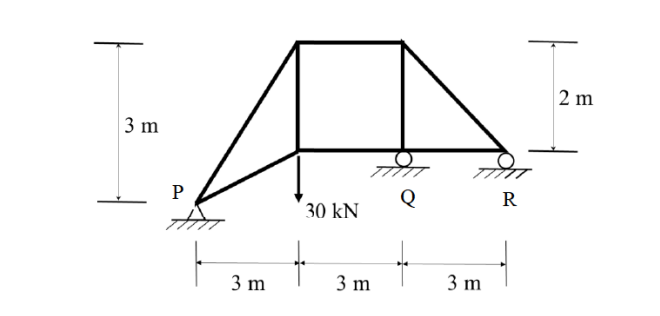
\includegraphics[width=0.5\columnwidth]{figs/q7.png}
\caption*{}
\label{fig:Q.7}
\end{figure}
\begin{enumerate}
\item $\brak{30,-30,30}kN$
\item $\brak{20,0,10}kN$
\item $\brak{10,30,-10}kN$
\item $\brak{0,60,-30}kN$
\end{enumerate}

\item Assuming that there is no possibility of shear buckling in the web, the maximum reduction permitted by IS 800-2007 in the (low-shear) design bending strength of a semi-compact steel section due to high shear is

\hfill{\brak{\text{GATE CE 2019}}}
\begin{enumerate}
\item zero
\item $25\%$
\item $50\%$
\item governed by the area of the flange
\end{enumerate}

\item In the reinforced beam section shown in the figure (not drawn to scale), the nominal cover provided at the bottom of the beam as per IS 456-2000, is

\hfill{\brak{\text{GATE CE 2019}}}
\begin{figure}
\centering
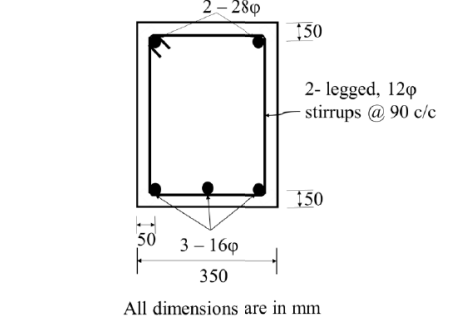
\includegraphics[width=0.5\columnwidth]{figs/q9.png}
\caption*{}
\label{fig:Q.9}
\end{figure}
\begin{enumerate}
\item $30mm$
\item $36mm$
\item $42mm$
\item $50mm$
\end{enumerate}

\item The interior angles of four triangles are given below:

\begin{table}[H]
\centering
\begin{tabular}{|c|c|}
\hline
Triangle & Interior angle\\
\hline
P & $85^\circ$, $50^\circ$, $45^\circ$\\
\hline
Q & $100^\circ$, $55^\circ$, $25^\circ$\\
\hline
R & $100^\circ$, $45^\circ$, $35^\circ$\\
\hline
S & $130^\circ$, $30^\circ$, $20^\circ$\\
\end{tabular}
\caption*{}
\label{tab:Q.10}
\end{table}
Which of the triangles are ill-conditioned and should be avoided in Triangulation surveys?

\hfill{\brak{\text{GATE CE 2019}}}
\begin{enumerate}
\item Both P and R
\item Both Q and R
\item Both P and S
\item Both Q and S
\end{enumerate}

\item The coefficient of average rolling friction of a road is $f_r$ and its grade is $+G\%$. If the grade of this road is doubled, what will be the percentage change in the braking distance $\brak{\text{for the design vehicle to come to a stop}}$ measured along the horizontal $\brak{\text{assume all other parameters are kept unchanged}}$?

\hfill{\brak{\text{GATE CE 2019}}}
\begin{enumerate}
\item $\dfrac{0.01\,G}{f_r + 0.02\,G} \times 100$
\item $\dfrac{f_r}{f_r + 0.02\,G} \times 100$
\item $\dfrac{0.02\,G}{f_r + 0.01\,G} \times 100$
\item $\dfrac{2f_r}{f_r + 0.01\,G} \times 100$
\end{enumerate}

\item An isolated concrete pavement slab of length $L$ is resting on a frictionless base. The temperature of the top and bottom fibre of the slab are $T_t$ and $T_b$, respectively. Given: the coefficient of thermal expansion $= \alpha$ and the elastic modulus $= E$. Assuming $T_t > T_b$ and the unit weight of concrete as zero, the maximum thermal stress is calculated as

\hfill{\brak{\text{GATE CE 2019}}}
\begin{enumerate}
\item $L\alpha(T_t - T_b)$
\item $E\alpha(T_t - T_b)$
\item $\dfrac{E\alpha(T_t - T_b)}{2}$
\item zero
\end{enumerate}

\item In a rectangular channel, the ratio of the velocity head to the flow depth for critical flow condition, is

\hfill{\brak{\text{GATE CE 2019}}}
\begin{enumerate}
\item $\dfrac{1}{2}$
\item $\dfrac{2}{3}$
\item $\dfrac{3}{2}$
\item $2$
\end{enumerate}

\item If the path of an irrigation canal is below the bed level of a natural stream, the type of cross-drainage structure provided is

\hfill{\brak{\text{GATE CE 2019}}}
\begin{enumerate}
\item Aqueduct
\item Level crossing
\item Sluice gate
\item Super passage
\end{enumerate}

\item A catchment may be idealised as a rectangle. There are three rain gauges located inside the catchment at arbitrary locations. The average precipitation over the catchment is estimated by two methods: (i) Arithmetic mean ($P_A$), and (ii) Thiessen polygon ($P_T$). Which one of the following statements is correct?

\hfill{\brak{\text{GATE CE 2019}}}
\begin{enumerate}
\item $P_A$ is always smaller than $P_T$
\item $P_A$ is always greater than $P_T$
\item $P_A$ is always equal to $P_T$
\item There is no definite relationship between $P_A$ and $P_T$
\end{enumerate}

\item A retaining wall of height $H$ with smooth vertical backface supports a backfill inclined at an angle $\beta$ with the horizontal. The backfill consists of cohesionless soil having angle of internal friction $\phi$. If the active lateral thrust acting on the wall is $P_a$, which one of the following statements is TRUE?

\hfill{\brak{\text{GATE CE 2019}}}
\begin{enumerate}
\item $P_a$ acts at a height $H/2$ from the base of the wall and at an angle $\beta$ with the horizontal
\item $P_a$ acts at a height $H/2$ from the base of the wall and at an angle $\phi$ with the horizontal
\item $P_a$ acts at a height $H/3$ from the base of the wall and at an angle $\beta$ with the horizontal
\item $P_a$ acts at a height $H/3$ from the base of the wall and at an angle $\phi$ with the horizontal
\end{enumerate}

\item In a soil specimen, the total stress, effective stress, hydraulic gradient and critical hydraulic gradient are $\sigma$, $\sigma'$, $i$ and $i_c$ respectively. For initiation of quicksand condition, which one of the following statements is TRUE?

\hfill{\brak{\text{GATE CE 2019}}}
\begin{enumerate}
\item $\sigma' \neq 0$ and $i = i_c$
\item $\sigma' = 0$ and $i = i_c$
\item $\sigma' \neq 0$ and $i \neq i_c$
\item $\sigma = 0$ and $i = i_c$
\end{enumerate}

\item Which one of the following is a secondary pollutant?

\hfill{\brak{\text{GATE CE 2019}}}
\begin{enumerate}
\item Ozone
\item Carbon Monoxide
\item Hydrocarbon
\item Volatile Organic Carbon $\brak{\text{VOC}}$
\end{enumerate}

\item For a given loading on a rectangular plain concrete beam with an overall depth of \textit{500 mm}, the compressive strain and tensile strain developed at the extreme fibers are of the same magnitude of $2.5 \times 10^{-4}$. The curvature in the beam cross-section $\brak{\text{in } m^{-1}, \textit{round off to 3 decimal places}}$ is \underline{\hspace{3cm}}.

\hfill{\brak{\text{GATE CE 2019}}}

\item A completely mixed dilute suspension of sand particles having diameters 0.25, 0.35, 0.40, 0.45 and 0.50 mm are filled in a transparent glass column of diameter 10 cm and height 2.50 m. The suspension is allowed to settle without any disturbance. It is observed that all particles of diameter 0.35 mm settle to the bottom of the column in 30 s. For the same period of 30 s, the percentage removal $\brak{\textit{round off to integer value}}$ of particles of diameters 0.45 and 0.50 mm from the suspension is \underline{\hspace{3cm}}.

\hfill{\brak{\text{GATE CE 2019}}}

\item The maximum number of vehicles observed in any five minute period during the peak hour is 160. If the total flow in the peak hour is 1000 vehicles, the five minute peak hour factor $\brak{\textit{round off to 2 decimal places}}$ is \underline{\hspace{3cm}}.

\hfill{\brak{\text{GATE CE 2019}}}

\item A circular duct carrying water gradually contracts from a diameter of $30cm$ to $15cm$. The figure $\brak{\textit{not drawn to scale}}$ shows the arrangement of differential manometer attached to the duct.

\begin{figure}[H]
    \centering
    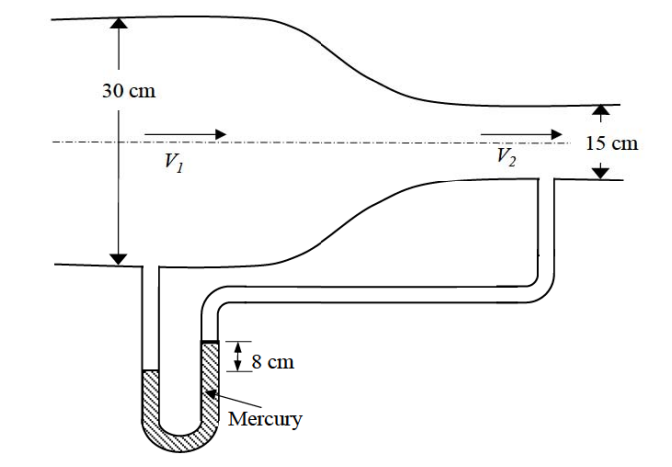
\includegraphics[width=0.5\linewidth]{figs/q22.png}
    \caption*{}
    \label{fig:Q.22}
\end{figure}
When the water flows, the differential manometer shows a deflection of $8cm$ of mercury $\brak{\textit{Hg}}$. The values of specific gravity of mercury and water are $13.6$ and $1.0$, respectively. Consider the acceleration due to gravity, $g=9.81m/s^2$. Assuming frictionless flow, the flow rate $\brak{\text{in } m^3/s,\textit{round off to 3 decimal places}}$ through the duct is \underline{\hspace{2cm}}.

\hfill{\brak{\text{GATE CE 2019}}}

\item The probability that the annual maximum flood discharge will exceed $25000 m^3/s$, at least once in next 5 years is found to be $0.25$. The return period of this flood event (in \textit{years, round off to 1 decimal place}) is \underline{\hspace{3cm}}

\hfill{\brak{\text{GATE CE 2019}}}

\item A soil has specific gravity of its solids equal to 2.65. The mass density of water is 1000 $kg/m^3$. Considering zero air voids and 10\% moisture content of the soil sample, the dry density (in $kg/m^3$, \textit{round off to 1 decimal place}) would be \underline{\hspace{3cm}}

\hfill{\brak{\text{GATE CE 2019}}}

\item A concentrated load of 500 $kN$ is applied on an elastic half space. The ratio of the increase in vertical normal stress at depths of 2 $m$ and 4 $m$ along the point of the loading, as per Boussinesq’s theory, would be \underline{\hspace{3cm}}

\hfill{\brak{\text{GATE CE 2019}}}

\section*{Q. 26-Q. 55 carry two marks each.}
\item Which one of the following is NOT a correct statement?

\hfill{\brak{\text{GATE CE 2019}}}
\begin{enumerate}
\item The function $\sqrt[3]{x}, (x>0)$, has the global maxima at $x = e$
\item The function $\sqrt[3]{x}, (x>0)$, has the global minima at $x = e$
\item The function $x^3$ has neither global minima nor global maxima
\item The function $|x|$ has the global minima at $x = 0$
\end{enumerate}
    
\item A one-dimensional domain is discretized into $N$ sub-domains of width $\Delta x$ with node numbers $i=0,1,2,3,\ldots,N$. If the time scale is discretized in steps of $\Delta t$, the forward-time and centered-space finite difference approximation at $i^{th}$ node and $n^{th}$ time step, for the partial differential equation $\frac{\partial v}{\partial t} = \beta \frac{\partial^2 v}{\partial x^2}$ is

\hfill{\brak{\text{GATE CE 2019}}}
\begin{enumerate}
\item $\frac{v_i^{(n+1)} - v_i^{(n)}}{\Delta t} = \beta \left[ \frac{v_{i+1}^{(n)} - 2 v_i^{(n)} + v_{i-1}^{(n)}}{(\Delta x)^2} \right]$
\item $\frac{v_{i+1}^{(n+1)} - v_i^{(n)}}{\Delta t} = \beta \left[ \frac{v_{i+1}^{(n)} - 2 v_i^{(n)} + v_{i-1}^{(n)}}{2 \Delta x} \right]$
\item $\frac{v_i^{(n)} - v_i^{(n-1)}}{\Delta t} = \beta \left[ \frac{v_{i+1}^{(n)} - 2 v_i^{(n)} + v_{i-1}^{(n)}}{(\Delta x)^2} \right]$  
\item $\frac{v_i^{(n)} - v_i^{(n-1)}}{2 \Delta t} = \beta \left[ \frac{v_{i+1}^{(n)} - 2 v_i^{(n)} + v_{i-1}^{(n)}}{2 \Delta x} \right]$
\end{enumerate}
    
\item A rectangular open channel has a width of $5m$ and a bed slope of 0.001. For a uniform flow of depth $2m$, the velocity is $2m/s$. The Manning's roughness coefficient for the channel is

\hfill{\brak{\text{GATE CE 2019}}}
\begin{enumerate}
\item 0.002
\item 0.017
\item 0.033
\item 0.050
\end{enumerate}

\item For the following statements:
\begin{itemize}
\item The lateral stress in the soil while being tested in an oedometer is always at-rest.
\item For a perfectly rigid strip footing at deeper depths in a sand deposit, the vertical normal contact stress at the footing edge is greater than that at its centre.
\item The corrections for overburden pressure and dilatancy are not applied to measured SPT-$N$ values in case of clay deposits.
\end{itemize}
The correct combination of the statements is

\hfill{\brak{\text{GATE CE 2019}}}
\begin{enumerate}
\item P -- TRUE; \quad Q -- TRUE; \quad R -- TRUE
\item P -- FALSE; \quad Q -- FALSE; \quad R -- TRUE
\item P -- TRUE; \quad Q -- TRUE; \quad R -- FALSE
\item P -- FALSE; \quad Q -- FALSE; \quad R -- FALSE
\end{enumerate}
    
\item Consider two functions: 
$x = \psi \ln \phi \quad \text{and} \quad y = \phi \ln \psi.$
Which one of the following is the correct expression for $\frac{\partial \psi}{\partial x}$?

\hfill{\brak{\text{GATE CE 2019}}}
\begin{enumerate}
\item $\displaystyle \frac{x \ln \psi}{\ln \phi \ln \psi - 1}$
\item $\displaystyle \frac{x \ln \phi}{\ln \phi \ln \psi - 1}$
\item $\displaystyle \frac{\ln \phi}{\ln \phi \ln \psi - 1}$
\item $\displaystyle \frac{\ln \psi}{\ln \phi \ln \psi - 1}$
\end{enumerate}

\item The cross-section of a built-up wooden beam as shown in the figure $\brak{\textit{not drawn to scale}}$ is subjected to a vertical shear force of $8kN$. The beam is symmetrical about the neutral axis $\brak{\text{N.A.}}$ shown, and the moment of inertia about N.A. is $1.5\times10^9mm^4$. Consisting that the nails at the location P are spaced longitudinally $\brak{\text{along the length of the beam}}$ at $60mm$ each of the nails at P will be subjeted to the shear force of

\hfill{\brak{\text{GATE CE 2019}}}
\begin{figure}[H]
\centering
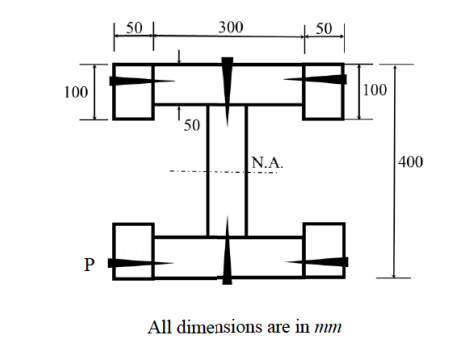
\includegraphics[width=0.5\columnwidth]{figs/q31.png}
\caption*{}
\label{fig:Q.31}
\end{figure}
\begin{enumerate}
\item $60N$
\item $120N$
\item $240N$
\item $480N$
\end{enumerate}

\item The rigid-jointed plane frame QRS shown in the figure is subjected to a load $P$ at the joint R. Let the axial deformations in the frame be neglected. If the support S undergoes a settlement of $\Delta=\frac{PL^3}{\beta El}$, the vertical reaction at the support S will become zero when $\beta$ is equal to

\hfill{\brak{\text{GATE CE 2019}}}
\begin{figure}[H]
\centering
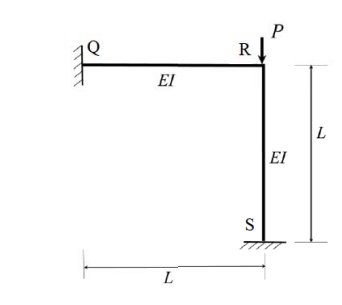
\includegraphics[width=0.5\columnwidth]{figs/q32.png}
\caption*{}
\label{fig:Q.32}
\end{figure}
\begin{enumerate}
\item $0.1$
\item $3.0$
\item $7.5$
\item $48.0$
\end{enumerate}

\item If the section shown in the figure turns from fully-elastic to fully-plastic, the depth of neutral axis $\brak{\text{N.A.}}$, $\vec{y}$, decreases by

\hfill{\brak{\text{GATE CE 2019}}}
\begin{figure}[H]
\centering
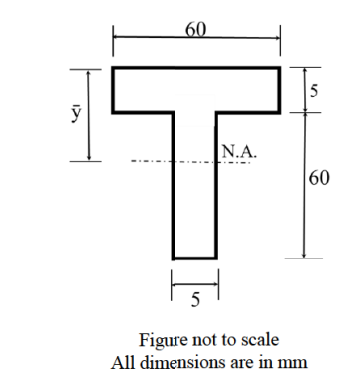
\includegraphics[width=0.5\columnwidth]{figs/q33.png}
\caption*{}
\label{fig:Q.33}
\end{figure}
\begin{enumerate}
\item $10.75mm$
\item $12.25mm$
\item $13.75mm$
\item $15.25mm$
\end{enumerate}

\item Sedimentation basin in a water treatment plant is designed for a flow rate of $0.2m^3/s$. The basin is rectangular with a length of $32m$, width of $8m$, and depth of $4m$. Assume that the settling velocity of these particles is governed by the Stokes' law. Given: density of the particles $=2.5g/cm^3$; density of water $=1g/cm^3$; dynamic viscosity of water $=0.01g/(cm.s)$; gravitational acceleration $=980cm/s^2$ If the incoming water contains particles of diameter $25\mu m$ $\brak{\text{spherical and uniform}}$, the removal efficiency of these particles is:

\hfill{\brak{\text{GATE CE 2019}}}
\begin{enumerate}
\item 51\%
\item 65\%
\item 78\%
\item 100\%
\end{enumerate}

\item A survey line was measured to be $285.5m$ with a tape having a nominal length of $30m$. On checking, the true length of the tape was found to be $0.05m$ too short. If the line lay on a slope of 1 in 10, the reduced length $\brak{\text{horizontal length}}$ of the line for plotting of survey work would be:

\hfill{\brak{\text{GATE CE 2019}}}
\begin{enumerate}
\item $283.6m$
\item $284.5m$
\item $285.0m$
\item $285.6m$
\end{enumerate}

\item A $16mm$ thick gusset plate is connected to the $12mm$ thick flange plate of an I-section using fillet welds on both sides as shown in the figure $\brak{\textit{not drawn to scale}}$. The gusset plate is subjected to a point load of $350kN$ acting at a distance of $100mm$ from the flange plate. Size of fillet weld is $10mm$.

\begin{figure}[H]
\centering
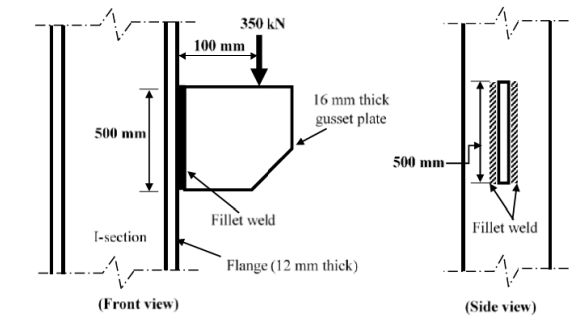
\includegraphics[width=0.5\columnwidth]{figs/q36.png}
\caption*{}
\label{fig:Q.36}
\end{figure}
The maximum resultant stress $\brak{\text{in }MPa,\textit{round off to 1 decimal place}}$ on the fillet weld along the vertical plane would be \underline{\hspace{2cm}}

\hfill{\brak{\text{GATE CE 2019}}}

\item The network of a small construction project awarded to a contractor is shown in the following figure. The normal duration, crash duration, normal cost, and crash cost of all the activities are shown in the table. The indirect cost incurred by the contractor is $INR 5000$ per day.

\begin{figure}[H]
\centering
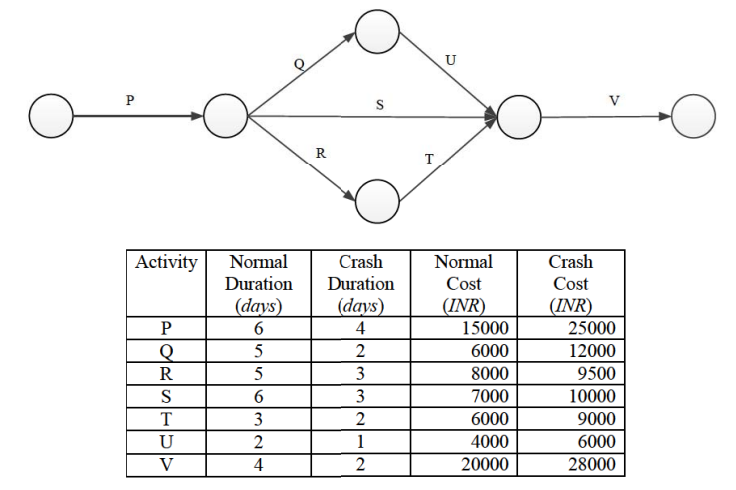
\includegraphics[width=0.5\columnwidth]{figs/q37.png}
\caption*{}
\label{fig:Q.37}
\end{figure}
If the project is targeted for the completion in 16 days, the total cost $\brak{\text{in }\textit{INR}}$ to be incurred by the contractor would be \underline{\hspace{2cm}}

\hfill{\brak{\text{GATE CE 2019}}}

\item A box measuring $50cm\times50cm\times50cm$ is filled to the top with dry coarse aggregate of mass $187.5kg$. The water absorption and specific gravity of the aggregate are $0.5\%$ and 2.5, respectively. The maximum quantity of water $\brak{\text{in kg,}\textit{round off to 2 decimal places}}$ required to fill the box completely is \underline{\hspace{2cm}}

\hfill{\brak{\text{GATE CE 2019}}}

\item A portal frame shown in figure $\brak{\textit{not drawn to scale}}$ has a hinge support at joint R. A point load of $50kN$ is acting at joint R in the horizontal direction. The flexular rigidity, $EI$, of each member is $10^6kNm^2$. Under the applied load, the horizontal displacement $\brak{\text{in mm, round off to 1 decimal point}}$ of joint R would be \underline{\hspace{2cm}}

\hfill{\brak{\text{GATE CE 2019}}}
\begin{figure}[H]
\centering
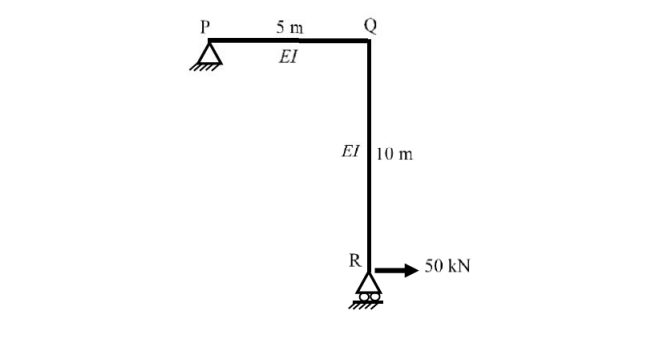
\includegraphics[width=0.5\columnwidth]{figs/q39.png}
\caption*{}
\label{fig:Q.39}
\end{figure}

\item A sample of air analysed at $0^\circ$C and $1atm$ pressure is reported to contain $0.02 ppm \brak{\text{parts per million}}$ of $NO_2$. Assume the gram molecular mass of $NO_2$ as 46 and its volume at $0^\circ$C and $1atm$ pressure as $22.4 litres$ per mole. The equivalent $NO_2$ concentration $\brak{\text{in }\textit{microgram per cubic meter, round off to 2 decimal places}}$ would be \underline{\hspace{2cm}}.

\hfill{\brak{\text{GATE CE 2019}}}

\item A $0.80 \, m$ deep bed of sand filter $\brak{\text{length 4m and width 3m}}$ is made of uniform particles $\brak{\text{diameter = 0.40mm, specific gravity = 2.65, shape factor = 0.85}}$ with bed porosity of 0.4. The bed has to be backwashed at a flow rate of $3.60m^3/min$. During backwashing, if the terminal settling velocity of sand particles is $0.05 m/s$, the expanded bed depth $\brak{\text{in m}, \textit{round off to 2 decimal places}}$ is \underline{\hspace{2cm}}.

\hfill{\brak{\text{GATE CE 2019}}}

\item A wastewater is to be disinfected with $35 \, mg/L$ of chlorine to obtain 99\% kill of micro-organisms. The number of micro-organisms remaining alive ($N_t$) at time $t$, is modelled by $N_t = N_0 e^{-kt}$
where $N_0$ is number of micro-organisms at $t = 0$, and $k$ is the rate of kill. The wastewater flow rate is $36 m^3/h$, and $k = 0.23 min^{-1}$. If the depth and width of the chlorination tank are $1.5 m$ and $1.0 m$, respectively, the length of the tank $\brak{\text{in m}, \textit{round off to 2 decimal places}}$ is \underline{\hspace{2cm}}.

\hfill{\brak{\text{GATE CE 2019}}}

\item A staff is placed on a benchmark (BM) of reduced level (RL) $100.000 m$ and a theodolite is placed at a horizontal distance of 50 m from the BM to measure the vertical angles. The measured vertical angles from the horizontal at the staff readings of $0.400m$ and $2.400m$ are found to be the same. Taking the height of the instrument as $1.400 m$, the RL (in m) of the theodolite station is \underline{\hspace{2cm}}.

\hfill{\brak{\text{GATE CE 2019}}}

\item Consider the ordinary differential equation $x^2 \frac{d^2 y}{dx^2} - 2x \frac{dy}{dx} + 2y = 0$. Given the values of $y(1) = 0$ and $y(2) = 2$, the value of $y(3)$ $\brak{\text{round off to 1 decimal place}}$ is \underline{\hspace{2cm}}.

\hfill{\brak{\text{GATE CE 2019}}}

\item Average free flow speed and the jam density observed on a road stretch are $60 km/h$ and $120 \, vehicles/km$, respectively. For a linear speed-density relationship, the maximum flow on the road stretch $\brak{\text{in} \textit{vehicles/h}}$ is \underline{\hspace{2cm}}.

\hfill{\brak{\text{GATE CE 2019}}}

\item Traffic on a highway is moving at a rate of $360 \, vehicles \, per \, hour$ at a location. If the number of vehicles arriving on this highway follows Poisson distribution, the probability $\brak{\textit{round off to 2 decimal places}}$ that the headway between successive vehicles lies between 6 and 10 seconds is \underline{\hspace{2cm}}.

\hfill{\brak{\text{GATE CE 2019}}}

\item A parabolic vertical curve is being designed to join a road of grade $+5\%$ with a road of grade $-3\%$. The length of the vertical curve is $400 \, m$ measured along the horizontal. The vertical point of curvature (VPC) is located on the road of grade $+5\%$. The difference in height between VPC and vertical point of intersection (VPI) $\brak{\text{in m}, \textit{round off to the nearest integer}}$ is \underline{\hspace{2cm}}.

\hfill{\brak{\text{GATE CE 2019}}}

\item Tie bars of $12 mm$ diameter are to be provided in a concrete pavement slab. The working tensile stress of the tie bars is $230 MPa$, the average bond strength between a tie bar and concrete is $2 MPa$, and the joint gap between the slabs is $10 mm$. Ignoring the loss of bond and the tolerance factor, the design length of the tie bars $\brak{\text{in mm}, \textit{round off to the nearest integer}}$ is \underline{\hspace{2cm}}.

\hfill{\brak{\text{GATE CE 2019}}}

\item The hyetograph of a storm event of duration 140 minutes is shown in the figure.

\begin{figure}[H]
\centering
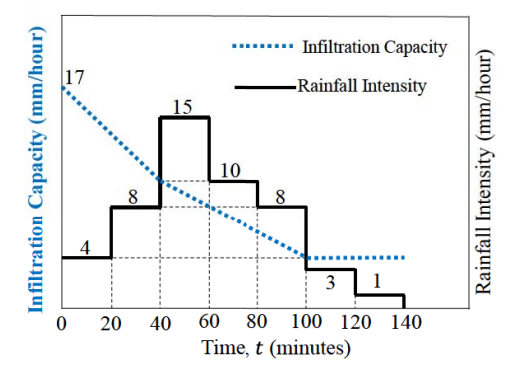
\includegraphics[width=0.5\columnwidth]{figs/q49.png}
\caption*{}
\label{fig:Q.49}
\end{figure}
The infiltration capacity at the start of this event $\brak{t=0}$ is $17mm/hour$, which linearly decreases to $10mm/hour$ after 40 minutes duration. As the event progresses, the infiltration rate further drops down linearly to attain a value of $4mm/hour$ at $t=100 minutes$ and remains constant thereafter till the end of the storm event. The value of te infiltration index, $\phi\brak{\text{in }\textit{mm/hour,round off to 2 decimal places}}$, is \underline{\hspace{2cm}}

\hfill{\brak{\text{GATE CE 2019}}}

\item  Two water reservoirs are connected by a siphon (running full) of total length $5000 m$ and diameter of $0.10 m$, as shown below $\brak{\textit{figure not drawn to scale}}$.

\begin{figure}[H]
\centering
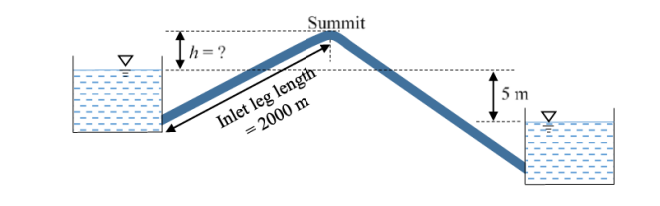
\includegraphics[width=0.5\columnwidth]{figs/q50.png}
\caption*{}
\label{fig:Q.50}
\end{figure}
The inlet leg length of the siphon to its summit is $2000 m$. The difference in the water surface levels of the two reservoirs is $5 m$. Assume the permissible minimum absolute pressure at the summit of siphon to be $2.5 m$ of water when running full. Given: friction factor $f =0.02$ throughout, atmospheric pressure$ = 10.3m$ of water, and acceleration due to gravity $g=9.81mm/s^2$. Considering only major loss using Darcy-Weisbach equation, the maximum height of the summit of siphon from the water level of upper reservoir, h $\brak{\text{in m}, \textit{round off to 1 decimal place}}$ is \underline{\hspace{2cm}}

\hfill{\brak{\text{GATE CE 2019}}}

\item Consider a laminar flow in the $x$-direction between two infinite parallel plates $\brak{\text{Couette flow}}$. The lower plate is stationary and the upper plate is moving with a velocity of $1 \, cm/s$ in the $x$-direction. The distance between the plates is $5 \, mm$ and the dynamic viscosity of the fluid is $0.01 \, N \cdot s/m^2$. If the shear stress on the lower plate is zero, the pressure gradient, $\dfrac{\partial p}{\partial x}$ $\brak{\text{in }N/m^2 \, per \, m, \textit{round off to 1 decimal place}}$ is \underline{\hspace{2cm}}.

\hfill{\brak{\text{GATE CE 2019}}}

\item A reinforced concrete circular pile of $12 \, m$ length and $0.6 \, m$ diameter is embedded in stiff clay which has an undrained unit cohesion of $110 \, kN/m^2$. The adhesion factor is $0.5$. The Net Ultimate Pullout (uplift) Load for the pile $\brak{in \, kN, \textit{round off to 1 decimal place}}$ is \underline{\hspace{2cm}}.

\hfill{\brak{\text{GATE CE 2019}}}

\item A granular soil has a saturated unit weight of $20 kN/m^3$ and an effective angle of shearing resistance of $30^\circ$. The unit weight of water is $9.81 kN/m^3$. A slope is to be made on this soil deposit in which the seepage occurs parallel to the slope up to the free surface. Under this seepage condition for a factor of safety of 1.5, the safe slope angle $\brak{\text{in degree, }\textit{round off to 1 decimal place}}$ would be \underline{\hspace{2cm}}.

\hfill{\brak{\text{GATE CE 2019}}}

\item A $3m \times 3m$ square precast reinforced concrete segment is to be installed by pushing them through an existing railway embankment for making an underpass as shown in the figure. A reaction arrangement using precast PCC blocks placed on the ground is to be made for the jacks.  

\begin{figure}[H]
    \centering
    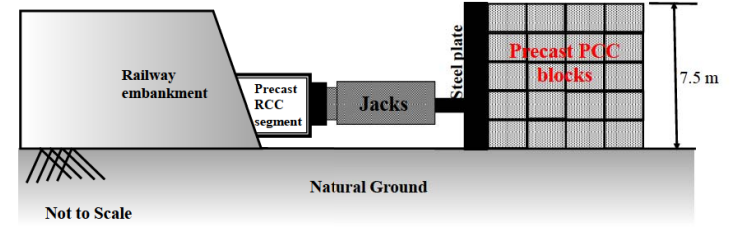
\includegraphics[width=0.5\columnwidth]{figs/q54.png}
    \caption*{}
    \label{fig:Q.54}
\end{figure}
At each stage, the jacks are required to apply a force of $1875 \, kN$ to push the segment. The jacks will react against the rigid steel plate placed against the reaction arrangement. The footprint area of reaction arrangement on natural ground is $37.5 \, m^2$. The unit weight of PCC block is $24 \, kN/m^3$. The properties of the natural ground are: $c = 17 \, kPa, \, \phi = 25^\circ, \text{and } \gamma = 18 \, kN/m^3$ Assuming that the reaction arrangement has rough interface and has the same properties as that of soil, the factor of safety (\textit{round off to 1 decimal place}) against shear failure is \underline{\hspace{2cm}}.

\hfill{\brak{\text{GATE CE 2019}}}

\item A square footing of $4m$ side is placed at $1m$ depth in a sand deposit. The dry unit weight $\brak{\gamma}$ of sand is $15kN/m^3$. This footing has an ultimate bearing capacity factor: $N_\gamma=18.75$. This footing is placed at a depth of $2m$ in the same soil deporit. For a factor of safety of $3.0$ as per Terzaghi's Theory, the safe bearing capacity $\brak{\text{in kPa}}$ of this footing would be \underline{\hspace{2cm}}

\hfill{\brak{\text{GATE CE 2019}}}
\end{enumerate}

\section*{END OF THE QUESTION PAPER}

\end{document}
